%% ============================================================
%%  Journal manuscript draft for Artificial Intelligence and Law
%%  Paper A: statutory domain-adaptive pretraining
%% ============================================================
\documentclass[pdflatex,sn-basic]{sn-jnl}

\usepackage{amsmath}
\usepackage{amssymb}
\usepackage{booktabs}
\usepackage{array}
\usepackage{enumitem}
\usepackage{algorithm}
\usepackage{algpseudocode}
\usepackage{placeins}
\usepackage{xurl}
\hypersetup{hypertexnames=false}
\providecommand{\doi}[1]{}
\renewcommand{\doi}[1]{%
  \href{https://doi.org/#1}{\mbox{\nolinkurl{https://doi.org/#1}}}}

\algrenewcommand\algorithmicrequire{\textbf{Input:}}
\algrenewcommand\algorithmicensure{\textbf{Output:}}
\algnewcommand{\LineComment}[1]{\hfill \(\triangleright\) \textit{#1}}

\graphicspath{{plots/}}
\raggedbottom

\begin{document}

\title[DAPT for Statutory Question Answering]{Domain-Adaptive Pretraining for
Statutory Question Answering: Evidence from Authentic, Synthetic, and Mixed
Legal Text}

\author[1]{\fnm{M. Mohaiminul} \sur{Islam}}
\email{niloy@students.sau.ac.in}

\author*[1]{\fnm{Muhammad} \sur{Abulaish}, \textit{SMIEEE}}
\email{abulaish@ieee.org}

\affil*[1]{\orgdiv{Department of Computer Science and Engineering},
\orgname{South Asian University},
\orgaddress{\city{New Delhi}, \country{India}}}




\abstract{Statutory question answering requires models to extract precise spans
from structured legal text. Domain-adaptive pretraining (DAPT) adds statutory
exposure, but better masked language model fit may not improve extraction. We test this with InLegalBERT and
IndicIPR-QA, an English benchmark covering seven Indian intellectual property
Acts. The main comparison fixes DAPT at 100 optimiser updates with 10 warmup
updates. Across five seeds, we compare authentic statutory text, synthetic text
generated from task questions and contexts, a mixture of the two, and no
additional DAPT. Mean test F1 is 85.86 without DAPT, 85.85 with authentic text,
85.91 with synthetic text, and 85.58 with mixed text. A condition test with
seed as a block detects no difference (\(p=0.706\)), and all paired
95\% intervals include zero. An earlier comparison trained for three epochs
gives the same general result despite unequal update counts. Masked language
model diagnostics improve without a matching extraction gain. Comparisons
using 25\% and 50\% of the answer labels do not establish that adaptation
becomes more beneficial as labelled data decrease. Under the tested
benchmark, encoder, corpus construction, and short adaptation budget, DAPT does
not reliably improve extraction. Legal DAPT evaluations should report language
model fit and task performance separately, alongside update counts, corpus
provenance, and seed uncertainty.}

\keywords{Legal NLP, Domain-adaptive pretraining, Extractive question answering,
Synthetic text, Statutory language, Indian intellectual property law}
\maketitle
\clearpage% Keep the opening heading separate from the title/abstract page.

\section{Introduction}\label{sec:intro}

Legal extractive question answering (QA) requires a reader to identify an
answer span in a source paragraph. Statutes contain enumerated clauses,
conditions, exceptions, and institutional terminology. A model may recognise
this language yet select a span that omits a qualification or extends into
an adjacent clause. Additional exposure to statutory text is therefore a
plausible adaptation strategy, but improved language model fit need not
improve the final answer.

Domain-adaptive pretraining (DAPT) continues a pretrained model's
self-supervised training on domain text
\citep{gururanganDontStopPretraining2020}. Legal domain encoders already
provide substantial legal language exposure
\citep{chalkidisLEGALBERTMuppetsStraight2020,paul2023pre}.
Here, DAPT is an umbrella term for the masked language model continuation stage.
The synthetic and mixed routes use continued pretraining informed by the task.
They are not adaptation based on domain text alone because their corpora use
benchmark questions and contexts, although they exclude answer strings and
offsets.
The question here is narrower than whether legal pretraining helps a generic
encoder: does additional statutory adaptation targeted to the benchmark improve
an InLegalBERT reader after the same supervised transfer and fine-tuning stages?

The choice of adaptation text complicates this comparison. Authentic
provisions retain statutory wording, whereas generated passages can extend
the adaptation pool without adding answer labels. Their combination may
change vocabulary, drafting patterns, and repetition. Corpus size, token
exposure, optimisation, and checkpoint selection can also differ. A high
score from one adapted checkpoint cannot identify which factor produced it.

The analysis uses IndicIPR-QA, a benchmark of 4,462 question--answer
pairs over seven Indian intellectual property Acts. Its construction and
validation are described in a separate accepted resource paper
\citep{anonymous2026indiciprbenchmark}. The present study holds the annotated
source paragraph available and studies reader adaptation; provision retrieval
is outside its scope. The evidence contains 62 independently trained readers.
It includes a comparison with equal update counts on the full dataset, an
earlier comparison trained for three epochs, a control written in statutory
style, and controls for the fraction of answer labels.

The study addresses four research questions:
\begin{description}[leftmargin=1.8cm,style=nextline]
\item[RQ1: Efficacy.] Under the executed training recipe, does additional
statutory DAPT improve the otherwise fixed InLegalBERT--SQuAD--IndicIPR-QA route?
\item[RQ2: Composition.] Under an MLM schedule with equal update counts, do authentic,
synthetic, and mixed adaptation corpora yield distinguishable answer extraction
performance on the full dataset across training seeds?
\item[RQ3: Target alignment.] Does synthetic text seeded by the target task
outperform an untargeted synthetic control written in statutory style?
\item[RQ4: Answer label fraction.] Does the DAPT effect change when final
IndicIPR-QA fine-tuning uses answer labels from fewer training sections?
\end{description}

The contribution is an empirical audit rather than a new encoder architecture.
First, a post hoc sensitivity comparison across five seeds matches MLM update counts,
warmup, and the learning rate schedule across authentic, synthetic, and mixed
DAPT. Second, a completed study with three training epochs, provenance checks,
and token budget
audits show which conclusions survive under a different exposure rule. Third,
paired controls for writing style and the fraction of answer labels test narrower explanations for
any apparent gain. Corpus, answer difficulty, and masked language model (MLM)
diagnostics support interpretation without substituting for downstream QA
evaluation.

This distinction is the main reason the absence of a detected effect is informative.
Validation MLM scores are often used to show that an encoder has adapted to a
domain, but improved reconstruction of statutory tokens is not itself evidence
of improved span extraction conditioned on the question. Evaluating both objectives
under the same downstream route tests whether the apparent language model
adaptation transfers to the task for which it is intended.

The test with equal update counts on the full dataset does not detect a
condition effect. The earlier test with three training epochs reaches the same
general finding. Synthetic DAPT gives a small positive contrast when fine-tuning
uses 50\% of the answer labels, but neither the interaction with the fraction of
answer labels nor the target alignment contrast establishes
a broader advantage. These are bounded findings: the adaptation budget is
small, the conditions with equal update counts process different numbers of nonpadding
tokens, and only one corpus sample is used per condition. The study therefore
distinguishes reproducible scores from stronger causal or legal conclusions.

The following sections situate the work, define the benchmark and executed
protocol, and report the completed results and diagnostics. The discussion
addresses legal interpretation and limits. Archived experiments and
validation only QA summaries are retained in the appendices rather than used
as substitutes for the final test comparisons.


\section{Related work}\label{sec:related}

\subsection{Domain-adaptive and synthetic continued pretraining}

BERT introduced bidirectional masked language model pretraining and showed that
the resulting encoder could be fine-tuned for extractive QA and language
inference with only small task specific output layers
\citep{devlinBERTPretrainingDeep2019}. Gururangan et al. then evaluated a second
pretraining phase on four domains and eight classification tasks. They reported
gains from domain-adaptive pretraining in both high- and low resource settings,
with further gains from adapting to unlabeled task data
\citep{gururanganDontStopPretraining2020}. Related domain specific models use
different training routes. SciBERT is pretrained on a corpus of scientific
publications, whereas BioBERT starts from BERT and continues pretraining on
PubMed abstracts and PubMed Central articles
\citep{beltagySciBERTPretrainedLanguage2019,leeBioBERTPretrainedBiomedical2020}.

Synthetic continued pretraining offers another route when only a small source
corpus is available. EntiGraph extracts salient entities from that corpus and
generates new text by connecting sampled entities
\citep{yangSyntheticContinuedPretraining2025}. TOP Training extracts entities
from a target medical extractive QA dataset, uses an LLM to generate texts that
contain those entities, and pretrains on the generated text
\citep{senguptaTOPTrainingTargetOrientedPretraining2025}. TOP Training is a
procedural precedent here, not the name of the present method. TRAIT combines
in domain data selection with task oriented synthetic passage generation for
continued pretraining, but evaluates advertising and mathematics rather than
law \citep{liangTaskOrientedInDomain2024}. This legal study uses rules and
keyphrases to guide unlabeled statutory style passages, then asks a different
question: under a specified downstream route and adaptation budget, are
authentic corpora, synthetic corpora informed by the task, and mixed corpora associated with
different results?

Kang et al. compare natural web text, rephrased text, generated textbooks, and
natural--synthetic mixtures across model sizes and data budgets. Their results
show that the effect of synthetic data depends on its type, mixture ratio, model
size, and budget \citep{kangSyntheticDataPretraining2025}. In a Taiwanese legal
study, continual pretraining improved domain knowledge but did not improve every
evaluated legal task \citep{chenContinualPretraining2025}. In a separate medical
study, seven adapted language models and two adapted vision--language models
were compared directly with their base models. Nearly all failed to improve
consistently in zero- and few-shot medical QA
\citep{jeongMedicalAdaptation2024}. These task specific results caution against
treating domain adaptation as an automatic downstream gain. They motivate the
present separation of MLM fit, fixed checkpoint QA performance, and
training seed variation.

\subsection{Legal language models and legal QA}

Greco and Tagarelli provide a systematic review of Transformer-based language
models across legal tasks and applications
\citep{grecoBringingOrderTransformer2024}.
Legal NLP has used both broad legal domain encoders and jurisdiction specific
models. LEGAL-BERT compares using BERT directly, continuing its pretraining on
legal corpora, and pretraining a legal model from scratch
\citep{chalkidisLEGALBERTMuppetsStraight2020}. Paul et al. continue the
pretraining of LegalBERT and CaseLawBERT on Indian legal text and also train a
custom vocabulary model from scratch \citep{paul2023pre}. LeXFiles is a
multinational English legal corpus, while MultiLegalPile contains 689 GB of
legal text from 17 jurisdictions in 24 languages
\citep{chalkidisLeXFilesLegalLAMA2023,niklausMultiLegalPile2024}. The Pile of
Law provides about 256 GB of open source English legal and administrative text
and treats responsible filtering as part of corpus construction
\citep{hendersonPileLaw2022}. Nair and Modani examine another design choice:
adding objectives that model two characteristics of legal language alongside
ordinary language model pretraining \citep{nairLegalCharacteristics2023}.

The value of legal domain and jurisdiction specific text is also
task dependent. Zheng et al. compare general and legal domain pretraining on
three legal tasks, including CaseHOLD. Their results associate larger gains
with greater task domain specificity and closer alignment between the
pretraining corpus and downstream task \citep{zhengWhenDoesPretraining2021}.
On the AusLaw citation benchmark, a 7B model pretrained only on 0.5 billion
Australian legal tokens slightly outperformed a model with the same backbone
that had been pretrained on 94 billion mixed jurisdiction legal tokens, after
both received the same citation instruction tuning. The authors present this
comparison as a preliminary experiment, so it supports a task specific result
rather than a general claim about legal pretraining \citep{han2026legal}.

Legal benchmarks also cover different tasks. LexGLUE combines several English
legal language understanding datasets in one evaluation suite
\citep{chalkidisLexGLUEBenchmarkDataset2022}. CUAD instead contains more than
13,000 expert annotations for identifying contract text that may require human
review \citep{hendrycksCUADExpertAnnotatedNLP2021}. These settings differ from
extractive QA over statutes.

Recent work in \emph{Artificial Intelligence and Law} covers several related but
distinct QA settings. Yuan et al. use GPT-3 to generate questions for a public
legal question bank and compare machine generated with human written questions
\citep{yuan2024bringing}. DiscoLQA evaluates discourse based, zero-shot answer
retrieval over six European norms \citep{sovrano2025discolqa}. Italiani et al.
generate synthetic legal context--question--answer triples with a frozen LLM
and use them to train smaller supervised models in a retrieval based setting
\citep{italiani2025enhancing}. AILQA evaluates retrieval augmented QA for Indian
legal material with automatic metrics and expert legal feedback, and also
reports an All India Bar Examination evaluation \citep{nigam2026ailqa}. These
papers address different data, outputs, and evaluation protocols. The present
paper focuses more narrowly on how reader pretraining affects extractive QA
when the annotated statutory paragraph is supplied.

\subsection{Synthetic text as adaptation material}

Italiani et al. identify the cost of carefully annotated legal QA data as a
barrier and use a frozen LLM to generate labelled examples for supervised
student model training \citep{italiani2025enhancing}. This paper uses synthetic
text differently. The generated passages are not treated as additional gold QA
labels and are not used to teach the model a particular answer. They are used
only during MLM pretraining, where the task is to reconstruct masked tokens from
local context. This distinction matters because a synthetic passage may still
provide useful adaptation text even when it has not been verified as a statement
of law.

The distinction also creates a different failure mode. Synthetic passages may
carry legal vocabulary and statutory form, but they may also carry generator
artifacts, repeated templates, or simplified legal structure. A strong
downstream result after synthetic DAPT would therefore not, by itself, show that
the model learned authentic legal reasoning. It could reflect useful lexical
coverage, regularisation, or accidental alignment with the benchmark's question
style. The corpus composition question has to be measured with controls rather
than inferred from one high performing route. Here, ``corpus composition''
denotes the combined provenance and properties of the constructed adaptation
corpus, including authenticity, generation process, lexical and length
distributions, and target conditioning. The design does not identify which
individual property would cause an observed difference.
More specifically, A versus S/M changes provenance and several correlated
linguistic properties; S versus Style tests target conditioning while holding
the generator and construction procedure broadly fixed; and token matching
controls approximate exposure scale. None of these comparisons independently
identifies lexical distribution, statutory structure, or factual accuracy as a
causal factor.

\subsection{Why corpus composition claims need audit}

DAPT experiments are especially vulnerable to confounding because the adaptation
stage is usually cheap to vary in several ways at once. A model may receive more
tokens, more duplicate passages, longer training, a different checkpoint
selection rule, or a different random seed, while the resulting table labels the
difference as ``authentic'' or ``synthetic'' text. This is a problem for
scientific interpretation even when all individual training runs are correctly
implemented. The correct comparison must specify the unit of exposure, the
eligibility rule for pretraining text, the amount of text, the training budget,
and the downstream pipeline. Repeated full pipeline seeds are particularly
important. Mosbach et al. show that changing only the random seed can produce
substantial variation when fine-tuning BERT, RoBERTa, and ALBERT on three GLUE
datasets \citep{mosbachStabilityBERT2021}.

The statutory setting makes this audit more important. Legal provisions contain
highly repeated formulae, numbered clauses, definitions, exceptions, and
institutional roles. Repetition is a real property of statutes, but it can also
make DAPT corpora look larger than they are if duplicate records are counted as
independent adaptation examples. The present paper therefore distinguishes
archived evidence matched by record count, the completed study with three
epochs and approximately matched token exposure, and the later sensitivity
comparison with equal update counts. The archive matched by record count does
not match token exposure. The study with three epochs
closely matches its initial token budget but not its update count. The
comparison with equal update counts matches the schedule but processes different
numbers of nonpadding tokens because the corpora have different length
distributions. None warrants an unrestricted causal claim about corpus
composition.


\section{Task and benchmark}\label{sec:task}

The task is extractive question answering with the gold statutory paragraph
provided. Each input is a pair \((q,c)\), where \(q\) is a natural language
question and \(c\) is the annotated source paragraph. The model predicts start
and end token positions, which the evaluator converts to a contiguous character
span in \(c\). Performance is reported as exact match (EM) and SQuAD style F1
at token level, as used in extractive QA
\citep{rajpurkarSQuAD100000Questions2016}. The evaluator lowercases text,
removes punctuation and normalizes whitespace; articles are retained.
Retrieval is outside the scope of
this manuscript.

The experiments use IndicIPR-QA, an extractive benchmark over seven Indian
intellectual property Acts: Patents, Trade Marks, Copyright, Designs,
Geographical Indications, Semiconductor Layout-Design, and Plant Varieties.
The dataset contains 4,462 question--answer pairs,
split into 3,710 training, 408 validation, and 344 test items. The split is
controlled at the statutory section level in the released benchmark so that
held out questions test unseen source sections rather than paraphrases of
training questions from the same section. Table~\ref{tab:data_summary}
summarises the dataset facts used by this paper.

Supplying the gold paragraph fixes upstream evidence identification and isolates
the question DAPT can directly affect: answer boundary prediction within a
source provision identified by the benchmark. Provision retrieval is evaluated
in separate work.

The evaluation target also matches the legal use case. A reader that extracts a
span from a statute must identify answer boundaries inside long, syntactically
dense provisions. Errors may involve omitted conditions, extra provisos,
truncated institutional roles, or confusion between a rule and an exception.
Token F1 describes partial token overlap, while exact match measures equality
with the normalised annotation. Neither directly measures whether an answer
preserves the provision's legal effect or all necessary qualifications.

\begin{table}[t]
\caption{Dataset facts required for the DAPT study. Benchmark construction and
human validation are reported in the companion resource paper; this manuscript
uses the benchmark as an evaluation instrument.}
\label{tab:data_summary}
\centering
\begin{tabular}{@{}lr@{}}
\toprule
Item & Value \\
\midrule
Legal domain & Indian intellectual property statutes \\
Statutory instruments & 7 Acts \\
QA pairs & 4,462 \\
Unique curated contexts & 1,116 \\
Train / validation / test & 3,710 / 408 / 344 \\
Mean question / context / answer length & 11.90 / 171.27 / 35.64 words \\
Evaluation setting & Gold statutory paragraph supplied \\
Primary metrics & EM and token F1 \\
\bottomrule
\end{tabular}
\end{table}


\FloatBarrier
\section{Executed Study Design}\label{sec:protocol}
\label{sec:method}

\subsection{Conditions and Replication}

All main study training/evaluation runs start from \texttt{law-ai/InLegalBERT}
\citep{paul2023pre}. Condition N omits additional MLM training; A uses authentic
training split provisions, S uses synthetic statutory style passages generated
from task questions and contexts, and M
mixes authentic and synthetic passages at approximately equal token shares.
The style control uses synthetic text matched by construction and written in statutory style
without conditioning on
the seven target Acts or their benchmark derived concepts.
Table~\ref{tab:final_protocol} summarises the executed design.

\begin{table}[!htbp]
\caption{Completed experiment inventory. D is the sensitivity analysis with equal update counts;
A--C are the earlier three-epoch studies. N, A, S, M, and Style denote
adaptation conditions. Reused readers are not counted twice.}
\label{tab:final_protocol}
\centering\small
\begin{tabular}{@{}>{\raggedright\arraybackslash}p{2.0cm}>{\raggedright\arraybackslash}p{5.7cm}>{\raggedright\arraybackslash}p{3.8cm}@{}}
\toprule
Experiment & Comparison & Independent reader runs \\
\midrule
D: equal updates & N/A/S/M; seeds 7, 42, 99, 123, 2026; N reused from A & 15 additional \\
A: three epochs & N/A/S/M; seeds 7, 42, 99, 123, 2026 & 20 \\
B: alignment & Style; seeds 7, 42, 99; paired with matching S runs from A & 3 additional \\
C: answer labels & N/A/S/M at 25\% and 50\%; seeds 7, 42, 99 & 24 additional \\
Evaluation & 408 validation and 344 test questions for every reader & 62 unique readers \\
MLM diagnostic & Base encoder and the 18 A/B adapted checkpoints & 19 encoders; validation only \\
\bottomrule
\end{tabular}
\end{table}

The experimental replication unit is a training seed, not an individual
prediction pooled across repeated readers. Experiment D was added after the
three-epoch study as a post hoc schedule sensitivity analysis. It reuses the
five N readers because N has no MLM stage, but trains new A, S, and M routes.
Experiment B reuses the corresponding S readers from A. Experiment C reuses
the SQuAD checkpoints from A that match both condition and seed and changes only the
final IPR fine-tuning data. The 62 unique readers require 33 MLM, 38 SQuAD,
and 62 IPR training stages. Corpus selection and answer label subsets are
fixed rather than resampled for each training seed.

\subsection{Synthetic Text and Source Provenance}\label{sec:provenance}

Seed extraction combines legal pattern rules with KeyBERT keyphrases
\citep{grootendorst2020keybert}, using context and question text rather than
answer strings or answer offsets. Gemma 3 models \citep{team2025gemma3}
generate unlabelled statutory style passages, not supervised QA pairs.
This corpus construction uses task information, although the subsequent MLM
objective is self-supervised.

The raw seed artifact requires a qualification. Its 5,859 records include
881 distinct exemplar contexts, three of which belong to the test split.
Those exemplars are associated with 19 seed entities. The saved propagation
audit checks primary and support seeds in the generation records and finds
that none of those 19 entities was sampled among the 1,282 distinct entities
used for generation. Consequently, no generated passage is removed by the
seed provenance quarantine. The evidence supports lack of propagation of this
raw artifact defect, not a claim that the original seed file was entirely
training only.

The archived accepted pool contains 13,211 distinct passages: 9,294 generated
by Gemma 3:12B and 3,917 by Gemma 3:27B. The final S and M corpora sample
only the audited 12B pool. Exact normalised held out context matching and
a 25-token overlap audit detect no held out reproduction in the eligible
synthetic pool. Shorter overlaps exist, as expected for repeated statutory
formulae; the checks do not prove semantic independence or reveal the
generator's original pretraining data.

The style only control uses the same 12B generator, decoding settings,
eight drafting style families and shared filtering code, with manually written
generic concepts and exemplars from untargeted statutory domains. It is not
conditioned on IndicIPR-QA seeds. This is a construction based control for
target conditioning, not a human validated semantic alignment measure.
Table~\ref{tab:generation_settings} records the common generation settings.

\begin{table}[!htbp]
\caption{Generation settings and scope of the automated checks. The final
pool seeded by the target task uses Gemma 3:12B; the two model archive is not the final
experimental mixture.}
\label{tab:generation_settings}
\centering\small
\begin{tabular}{@{}>{\raggedright\arraybackslash}p{3.1cm}>{\raggedright\arraybackslash}p{8.2cm}@{}}
\toprule
Component & Executed setting \\
\midrule
Target seed selection & Frequency ranked raw pool capped at 1,500 entries;
primary/support seed provenance audited as described in the text \\
Style families & Definition; registration; rights/remedies; authority/procedure;
conditions/compliance; penalty/enforcement; licensing/assignment; dispute/appeal \\
Generation backend & Local Ollama; Gemma 3:12B for final S, M and Style \\
Decoding & Temperature 0.40; top-\(p=0.85\); repeat penalty 1.12;
context length 4,096; maximum generated length 250 tokens \\
Output checks & Nonempty text, 70--280 words, at least two sentences,
required concept, and legal style lexical markers \\
Rejections & Prompt/placeholder leakage, markdown, question marks, bullet
format, prohibited openings, and severe repetition \\
Deduplication & Exact normalised text duplicates removed from merged pool \\
Not established & Legal correctness, doctrinal consistency, or suitability
of generated text as legal authority \\
\bottomrule
\end{tabular}
\end{table}

\subsection{Token Matching and the Executed Optimisation Budget}

A contains the 898 distinct contexts in the training split. S is sampled
to approximately A's token budget. M allocates approximately half of its
tokens to authentic text and half to a separately selected synthetic subset.
The corpus selection seed is 20260829. Token counts include special tokens
after truncation to 256 tokens and exclude padding. The same fixed A, S, and M
corpora are used in Experiments A and D. Table~\ref{tab:budgets} reports the
three-epoch exposure used in A--C.

\begin{table}[!htbp]
\caption{Adaptation corpora and three-epoch MLM budget used in Experiments
A--C. Tokens are counted per epoch. Updates cover three epochs; every condition
has 100 warmup updates.}
\label{tab:budgets}
\centering\small
\begin{tabular}{@{}lrrrr@{}}
\toprule
Condition & Records & Nonpadding tokens & Updates & Warmup \\
\midrule
A & 898 & 128,727 & 87 & 100 \\
S & 861 & 128,713 & 81 & 100 \\
M & 879 & 128,663 & 84 & 100 \\
Style & 858 & 128,723 & 81 & 100 \\
\bottomrule
\end{tabular}
\end{table}

Token totals differ by less than 0.05\%, but record counts and optimiser
updates are not matched. With batch size 8 and gradient accumulation 4,
three epochs produce 81--87 updates. All A--C MLM runs therefore finish during
the 100-update warmup rather than completing the nominal linear learning rate
schedule. Different update counts also imply different integrated
learning rate exposure.

Experiment D addresses this schedule difference. Each adapted route completes
exactly 100 optimiser updates, uses 10 warmup updates, reaches the configured
peak learning rate, and finishes the linear decay at zero. Table~\ref{tab:equal_update_budget}
reports the telemetry. Equal update counts do not give equal token exposure:
the mean processed total is about 445,757 tokens for A, 477,072 for S, and
460,828 for M. The differences follow from the fixed batch construction and
the corpora's different length distributions.

\begin{table}[!htbp]
\caption{Executed MLM budget with equal update counts in Experiment D. Token totals are
means and ranges across five seeds and exclude padding. N has no MLM stage.}
\label{tab:equal_update_budget}
\centering\small
\begin{tabular}{@{}lrrr@{}}
\toprule
Condition & Updates & Warmup & Processed nonpadding tokens \\
\midrule
A & 100 & 10 & 445,757 (444,219--447,947) \\
S & 100 & 10 & 477,072 (476,715--477,394) \\
M & 100 & 10 & 460,828 (460,181--461,490) \\
\bottomrule
\end{tabular}
\end{table}

Experiment D controls update count and learning rate trajectory, while
Experiment A controls the initial corpus token budget more closely. Together
they provide two bounded comparisons rather than a complete isolation of
corpus composition.

\subsection{Training and Checkpoint Selection}

Algorithm~\ref{alg:dapt} summarises the executed routes.
MLM uses the terminal checkpoint after either the three-epoch A--C schedule or
the 100-update D schedule, with no validation loss checkpoint selection. SQuAD
transfer and IPR fine-tuning
select the lowest validation loss checkpoint.
Table~\ref{tab:training_recipe} gives the executed hyperparameters.
The SQuAD~v1 subsets contain 20,000 training and 2,000 validation examples,
sampled with seed 42 and held fixed across conditions. Training seeds are
applied to the model and training data order.

Each planned route is represented by \(r=(d,s,f,b)\), where \(d\) is the
adaptation condition, \(s\) is the training seed, \(f\) is the percentage of
IPR answer labels used for final fine-tuning, and \(b\) is the MLM schedule.
The experiment plan contains only the combinations executed in Experiments
A--D.

\begin{algorithm}[!htbp]
\caption{Audited DAPT and reader evaluation procedure}
\label{alg:dapt}
\begin{algorithmic}[1]
\Require Experiment plan \(\mathcal{P}\), audited corpora \(\mathcal{C}_d\),
base encoder \(\theta_0\), fixed SQuAD subsets, and fixed IPR splits
\Ensure Per-route validation and locked-test predictions with
annotation-relative EM and F1 scores
\ForAll{routes \(r=(d,s,f,b)\in\mathcal{P}\)}
    \State \(\theta\gets\theta_0\); set training seed to \(s\)
    \If{\(d\neq N\)}
        \State \(\theta\gets\Call{MLMAdapt}{\theta,\mathcal{C}_d,b}\)
        \LineComment{three epochs or 100 updates}
        \State Retain the terminal MLM checkpoint
        \LineComment{no validation selection}
    \Else
        \State Retain \(\theta_0\)
        \LineComment{no additional DAPT}
    \EndIf
    \State \(\theta_{\mathrm{SQ}}\gets\Call{FineTuneSQuAD}{\theta}\)
    \State Select the lowest-validation-loss SQuAD checkpoint
    \State \(T_f\gets\Call{FixedIPRSubset}{f}\)
    \LineComment{\(f\in\{25,50,100\}\)}
    \State \(\theta_{\mathrm{IPR}}\gets
    \Call{FineTuneIPR}{\theta_{\mathrm{SQ}},T_f}\)
    \State Select the lowest-validation-loss IPR checkpoint
    \ForAll{\((q_i,c_i,a_i)\) in the validation split}
        \State \(\widehat{a}_i\gets
        \Call{Decode}{\theta_{\mathrm{IPR}},q_i,c_i}\)
        \LineComment{common span decoder}
        \State Score \(\widehat{a}_i\) against annotation \(a_i\)
    \EndFor
    \State Store validation results
    \State Verify the frozen test analysis lock
    \LineComment{no test-based selection}
    \ForAll{\((q_i,c_i,a_i)\) in the locked test split}
        \State \(\widehat{a}_i\gets
        \Call{Decode}{\theta_{\mathrm{IPR}},q_i,c_i}\)
        \LineComment{same span decoder}
        \State Score \(\widehat{a}_i\) against annotation \(a_i\)
    \EndFor
    \State Store test results separately
\EndFor
\State Pair conditions by seed and compute the specified contrasts
\end{algorithmic}
\end{algorithm}

\begin{table}[!htbp]
\caption{Executed training settings. Batch denotes per device batch size
times gradient accumulation. D denotes the sensitivity analysis with equal update counts; A--C
denote the earlier three-epoch studies.}
\label{tab:training_recipe}
\centering\small
\begin{tabular}{@{}lcccc@{}}
\toprule
Setting & MLM D & MLM A--C & SQuAD & IPR \\
\midrule
Maximum tokens & 256 & 256 & 384 & 384 \\
Window overlap & --- & --- & 128 & 128 \\
Budget & 100 updates & 3 epochs & 2 epochs & 3 epochs \\
Batch & \(8\times4\) & \(8\times4\) & \(16\times2\) & \(16\times2\) \\
Learning rate & \(2\times10^{-5}\) & \(2\times10^{-5}\) & \(3\times10^{-5}\) & \(2\times10^{-5}\) \\
Weight decay & 0.01 & 0.01 & 0.01 & 0.01 \\
Warmup updates & 10 & 100 & 200 & 50 \\
Scheduler & Linear & Linear & Linear & Linear \\
Checkpoint & Terminal & Terminal & Min.\ val.\ loss & Min.\ val.\ loss \\
\bottomrule
\end{tabular}
\end{table}

MLM masks tokens with probability 0.15. Training is CPU based without
half precision. Saved stage scripts and their hashes identify the executed
settings; the amended analysis record distinguishes these scripts from the
unrecoverable earlier runner version
(Section~\ref{sec:analysis_provenance}).

\subsection{Scope of Fine-Tuning with Fewer Answer Labels}\label{sec:reduced_design}

The 25\% and 50\% subsets sample statutory sections, stratified by Act, using
seed 20260829. They contain respectively 135 and 270 of 541 training sections,
yielding 942 and 1,852 of 3,710 QA pairs (25.39\% and 49.92\%).
Each fraction uses one fixed subset shared across conditions and training
seeds. The validation and test sets are unchanged.

These fractions reduce final supervised IPR fine-tuning, not all access to
the task resource. Adaptation corpora remain derived from the full eligible
training resource, including question derived generation seeds, and all
conditions retain SQuAD transfer. The experiment therefore tests reduced
fine-tuning with answer labels while broader task informed text remains available. It does
not measure a proportional reduction in question acquisition, annotation
cost, or total training compute. Seed uncertainty does not include variation
over independently drawn reduced answer label subsets.

\subsection{Decoding, Metrics and Statistical Comparisons}

The common decoder uses 384-token question--context windows with 128-token
overlap. It considers valid spans with start position no later than end,
imposes no additional answer length cap, and returns the literal source text
span with the highest summed start/end logit across windows.
Exact match (EM) and SQuAD style token F1 lowercase text, remove punctuation
and normalise whitespace, retaining articles. This is not identical to the official SQuAD
normalisation. Character Frequency overlap is not used as a paper metric.
All scores concern the benchmark annotation, not independently assessed legal
correctness.

The decoder uses the tokenizer's question/context sequence IDs and offset
mapping, considers context tokens only, masks spans with start position greater
than end position, and converts the winning token offsets into a literal
character slice of the original context. Spans cannot cross a window boundary;
overflow windows are mapped back to their source example and the highest raw
start plus end logit across windows is retained. No null answer option or
additional answer length cap is used.

For Experiment D, the condition comparison is a complete block analysis of
variance with training seed as the block. Pairwise confidence intervals use
the Student's \(t\) distribution over paired seed differences. Holm correction
covers the three DAPT versus N contrasts separately for EM and F1. This
analysis was specified and locked after validation review but before D test
evaluation; it remains a post hoc sensitivity study because D was designed
after the earlier A--C results.

Experiment A uses the same blocked analysis and applies Holm correction to all
six pairwise contrasts on the full dataset separately for each metric. Experiment C
applies Holm correction to the three DAPT versus N contrasts within each
fraction of answer labels and metric. The style contrast and the contrast over fractions of answer labels
interaction contrasts are reported with their unadjusted values. These
analyses do not constitute one study wide multiplicity correction.

\begin{samepage}
To test whether the DAPT contrast changes with the fraction of answer labels,
let \(Y_{d,f,s}\) denote test F1 for condition \(d\), label fraction \(f\), and
seed \(s\). Experiment C uses the seed-level interaction contrast
\[
\Delta_{d,f,s}
=
\left(Y_{d,f,s}-Y_{N,f,s}\right)
-
\left(Y_{d,100,s}-Y_{N,100,s}\right),
\]
for \(d\in\{A,S,M\}\), \(f\in\{25,50\}\), and
\(s\in\{7,42,99\}\). The mean, confidence interval, and paired test are
computed over the three seed-level values of \(\Delta_{d,f,s}\).
\end{samepage}
The 100\% reference is the three-epoch Experiment A route, not the later
Experiment D route with equal update counts.
A nonsignificant result is treated as a failure to detect an effect, not as
evidence of equivalence.
Intervals condition on the fixed test set, corpus selections and training
subsets. They do not capture all sources of dataset or source section
uncertainty. A clearly labelled post hoc sign flip sensitivity check is
reported separately in Section~\ref{sec:low_results}.

\FloatBarrier

\section{Results of the Completed Study}\label{sec:results}

Validation summaries are reported separately in Appendix~\ref{app:validation};
they are not substituted for test results. All 62 readers have saved
checkpoints and completed evaluations.

\subsection{Efficacy and Corpus Composition with Equal Update Counts}
\label{sec:equal_update_results}

Table~\ref{tab:equal_update_test} reports the main comparison with equal update counts on
the 344-question test set. Mean F1 is 85.86 for N, 85.85 for A, 85.91 for S,
and 85.58 for M. The seed blocked condition test gives
\(F(3,12)=0.474\), \(p=0.706\), and partial \(\eta^2=0.106\).
The corresponding EM test gives \(F(3,12)=0.245\), \(p=0.863\).

\begin{table}[!htbp]
\caption{Experiment D with equal update counts: test results on 344 questions. EM and F1
use the 0--100 scale; SD is the sample standard deviation across five seeds.}
\label{tab:equal_update_test}
\centering\scriptsize
\begin{tabular}{@{}lrr>{\raggedright\arraybackslash}p{4.4cm}@{}}
\toprule
Condition & Mean EM & Mean F1 $\pm$ SD & \shortstack[l]{DAPT--N F1 difference\\(95\% interval)} \\
\midrule
No DAPT & 65.76 & $85.86\pm1.08$ & --- \\
Authentic & 65.76 & $85.85\pm0.46$ & $-0.01\;[-1.34,1.32]$ \\
Synthetic & 65.47 & $85.91\pm0.84$ & $+0.05\;[-0.80,0.90]$ \\
Mixed & 65.29 & $85.58\pm0.75$ & $-0.28\;[-1.16,0.60]$ \\
\bottomrule
\end{tabular}
\end{table}

All three paired F1 intervals include zero, and all Holm adjusted
DAPT versus N \(p\)-values equal 1.00. The paired differences vary across
seeds. For example, S minus N ranges from $-0.70$ to $+1.10$ F1 points.
Figure~\ref{fig:equal_update_effects} shows the per seed scores and paired
intervals. The figure displays uncertainty around the observed effects; the
zero line is not an equivalence margin. The intervals also do not rule out
effects of practical interest. The widest one, for A minus N, extends from
$-1.34$ to $+1.32$ F1 points.

\begin{figure}[!htbp]
\centering
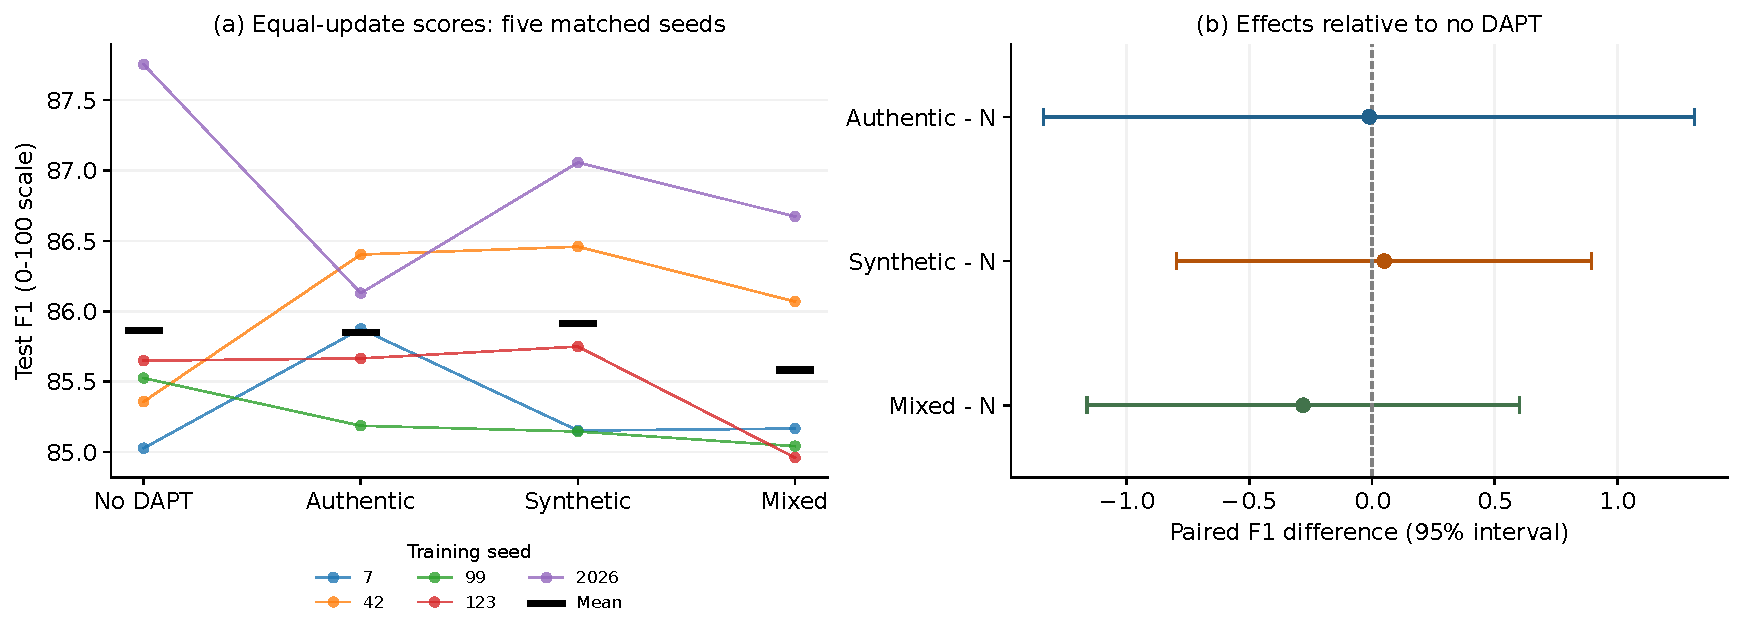
\includegraphics[width=\textwidth]{09_equal_update_full_data.pdf}
\caption{Experiment D with equal update counts. Left: test F1 for each of five matched
training seeds, with condition means marked. Right: paired DAPT minus N F1
differences and 95\% Student's \(t\) intervals. N uses the matching no DAPT
readers from Experiment A because it has no MLM stage.}
\label{fig:equal_update_effects}
\end{figure}

\paragraph*{Answers to RQ1 and RQ2.}
Under the schedule with equal update counts, the study does not detect a DAPT benefit on
the full dataset or a difference among authentic, synthetic, and mixed adaptation.
The absence of a detected effect is not evidence that the routes are equivalent. The result
applies to the tested 100-update schedule, fixed corpora, encoder, and
downstream route.

\subsection{Earlier Three-Epoch Experiments}

Table~\ref{tab:final_test} reports the earlier A--C test results. These
experiments retain the schedule of three epochs with approximately matched token exposure and
its unequal update counts. They provide schedule sensitivity, target alignment,
and controls for the fraction of answer labels rather than replacements for Experiment D.

\begin{table}[!htbp]
\caption{Earlier three-epoch A--C studies: test results on 344 questions. EM
and F1 use the 0--100 scale; SD is the sample standard deviation across seeds.}
\label{tab:final_test}
\centering
\small
\begin{tabular}{@{}llrrrr@{}}
\toprule
Experiment & Condition & IPR labels (\%) & Seeds & Mean EM & Mean F1 $\pm$ SD \\
\midrule
A & No DAPT & 100 & 5 & 65.76 & $85.86\pm1.08$ \\
A & Authentic & 100 & 5 & 65.58 & $85.75\pm0.59$ \\
A & Synthetic & 100 & 5 & 65.81 & $85.39\pm0.67$ \\
A & Mixed & 100 & 5 & 65.35 & $85.48\pm0.55$ \\
B & Style Only & 100 & 3 & 65.12 & $85.60\pm0.55$ \\
\midrule
C & No DAPT & 25 & 3 & 62.50 & $83.54\pm0.77$ \\
C & Authentic & 25 & 3 & 62.02 & $83.73\pm0.34$ \\
C & Synthetic & 25 & 3 & 62.21 & $83.89\pm0.65$ \\
C & Mixed & 25 & 3 & 61.43 & $83.73\pm0.88$ \\
C & No DAPT & 50 & 3 & 63.28 & $84.17\pm0.40$ \\
C & Authentic & 50 & 3 & 63.95 & $84.35\pm0.74$ \\
C & Synthetic & 50 & 3 & 63.76 & $84.60\pm0.44$ \\
C & Mixed & 50 & 3 & 63.08 & $84.53\pm0.64$ \\
\bottomrule
\end{tabular}
\end{table}

\subsubsection{Full Dataset Sensitivity with Matched Token Exposure}\label{sec:full_results}

Mean F1 is 85.86 for N, 85.75 for A, 85.39 for S and 85.48 for M.
The seed blocked test gives \(F(3,12)=0.635\), \(p=0.607\), and partial
\(\eta^2=0.137\). A, S and M differ from N by
\(-0.12\), \(-0.47\) and \(-0.38\) points, with paired 95\% intervals
\([-1.60,1.37]\), \([-1.41,0.47]\) and \([-2.01,1.24]\).
All six F1 contrasts on the full dataset have Holm adjusted \(p=1.00\).
The EM condition test is likewise not significant
(\(F(3,12)=0.108\), \(p=0.954\)).
Figure~\ref{fig:final_effects} shows the seed level scores and paired F1 effects.

\begin{figure}[!htbp]
\centering
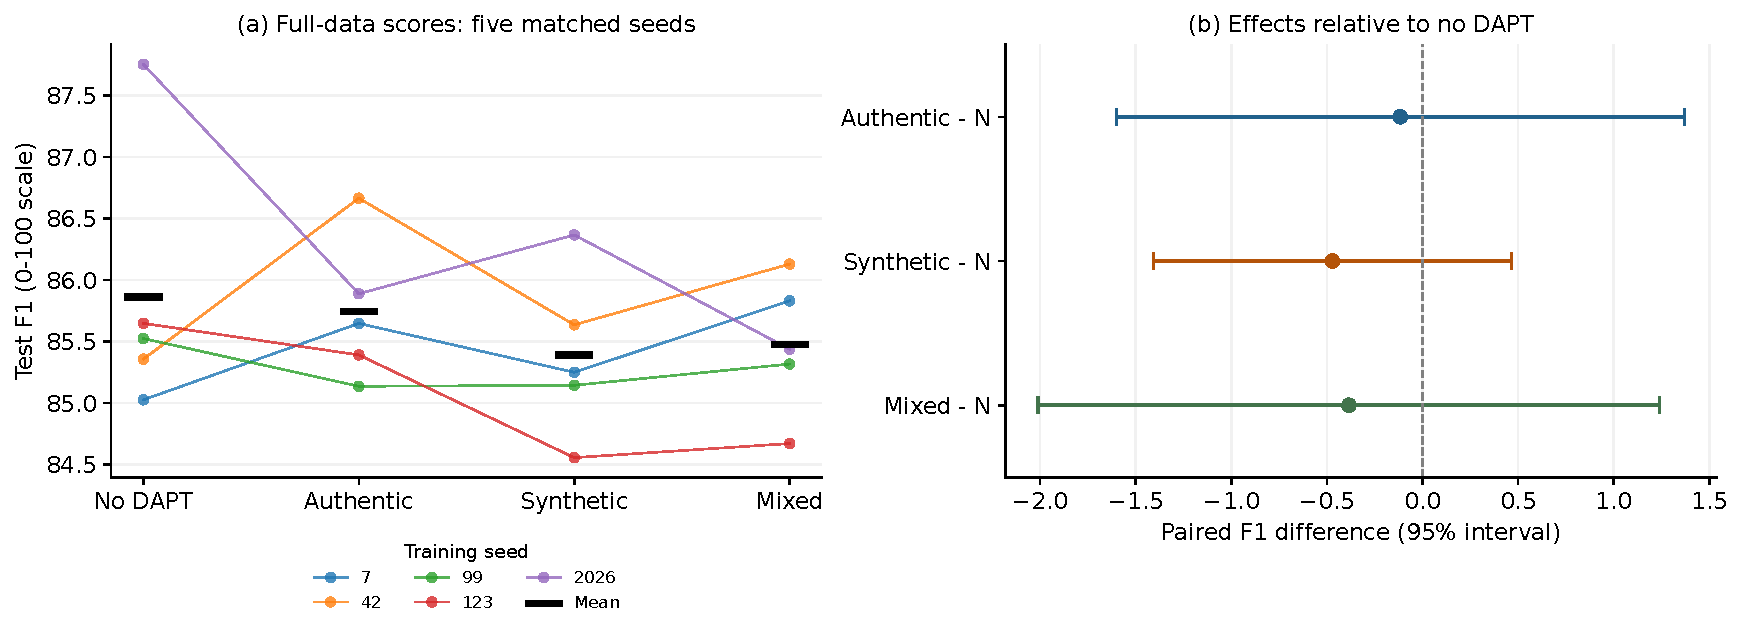
\includegraphics[width=\textwidth]{07_final_full_data.pdf}
\caption{Three-epoch Experiment A. Left: test F1 for each of five training
seeds, with matching seeds connected and condition means marked.
Right: paired DAPT minus N F1 differences and 95\% Student's \(t\) intervals.
The zero line denotes no difference, not an equivalence margin.}
\label{fig:final_effects}
\end{figure}

Experiment A also gives no detected condition effect. Because it uses unequal
update counts and ends during warmup, Experiment D provides the cleaner
schedule comparison.

\subsubsection{Target Alignment}\label{sec:alignment_results}

Using matching seeds 7, 42 and 99, S reaches 85.34 mean F1 and the
untargeted statutory style control reaches 85.60. The difference between S and
Style is \(-0.26\) points, with interval \([-1.32,0.80]\) and
uncorrected \(p=0.404\). This comparison uses the S mean across three seeds, not
the value across five seeds in the full dataset rows of Table~\ref{tab:final_test}.

\paragraph*{Answer to RQ3.}
The experiment does not detect a target alignment advantage over generic
statutory style adaptation at this budget. The control compares particular
corpus constructions; it does not establish that target specific concepts
are irrelevant or that generated text is legally accurate.

\subsubsection{Fine-Tuning with Fewer Answer Labels}\label{sec:low_results}

At 25\%, the three DAPT versus N F1 intervals include zero. At 50\%, a
preliminary synthetic versus no DAPT contrast of +0.43 F1 points is observed
under the paired-\(t\) analysis (interval \([0.30,0.56]\), within fraction
Holm adjusted \(p=0.014\)); the exact sign flip sensitivity check gives
\(p=0.25\).
A and M have positive sample differences of 0.18 and 0.35 points, but
their intervals include zero. Figure~\ref{fig:supervision_effects}
compares the effects at all three fractions using the same three seeds.

\begin{figure}[!htbp]
\centering
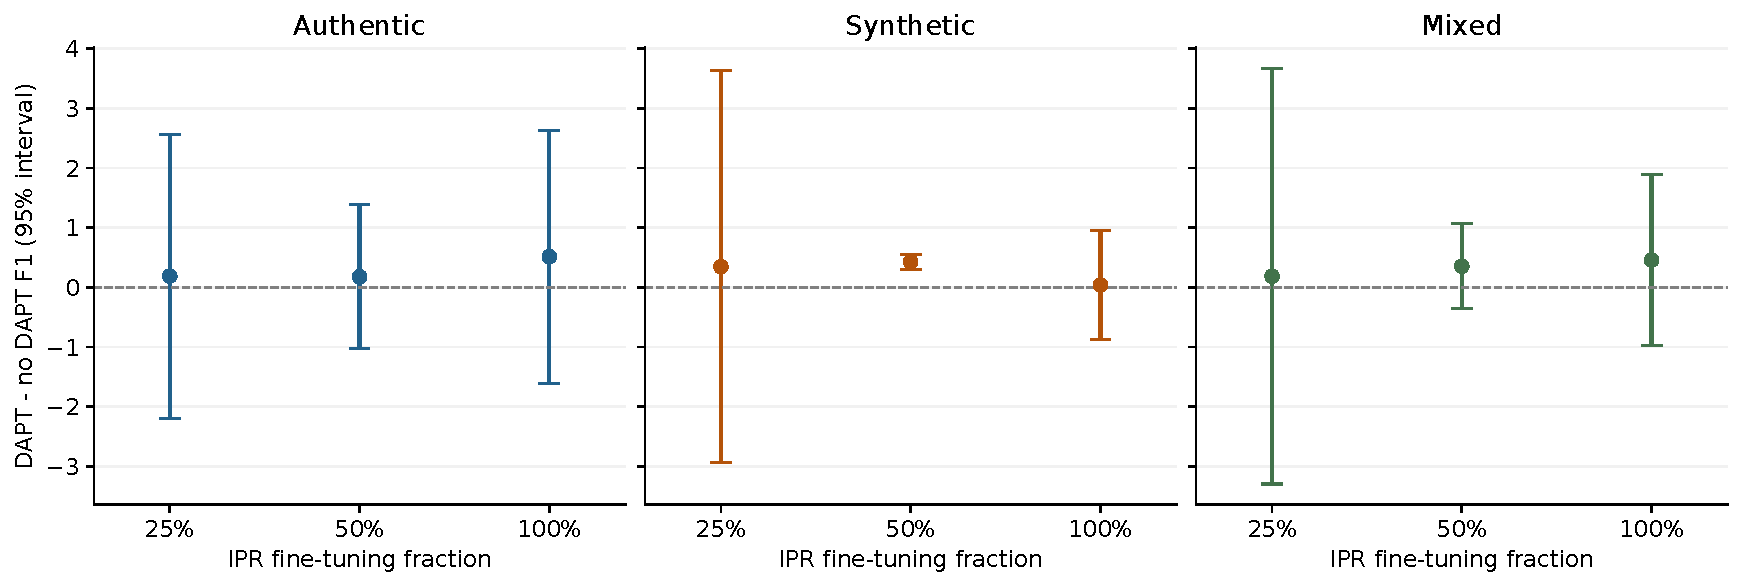
\includegraphics[width=\textwidth]{08_final_supervision.pdf}
\caption{DAPT minus N test F1 by final supervised fine-tuning fraction.
Points are paired mean differences and bars are 95\% Student's \(t\) intervals.
All panels use seeds 7, 42 and 99, including the 100\% comparison.
The 100\% point comes from the three-epoch Experiment A, not Experiment D.
Fractions refer to section sampled fine-tuning subsets, not total task resource
access. The panels do not establish an interaction with the fraction of answer labels.}
\label{fig:supervision_effects}
\end{figure}

The direct interaction comparison is important. For S,
\((S-N)_{50}-(S-N)_{100}=0.39\), with interval \([-0.59,1.36]\)
and unadjusted \(p=0.230\). At 25\%, the corresponding difference is
0.31, with interval \([-3.84,4.45]\), \(p=0.781\).
All six A/S/M interaction intervals contain zero
(Table~\ref{tab:interactions}). A significant contrast at one fraction and a
contrast that is not significant at another do not establish different effects.

The three differences between S and N at 50\% are 0.463, 0.369 and 0.452 points.
The narrow paired-\(t\) interval reflects their consistency but has only
two degrees of freedom. A post hoc exact two sided sign flip sensitivity
check gives \(p=0.25\), with only eight possible sign assignments.
This does not replace or invalidate the specified \(t\)-test calculation;
it illustrates the limited resolution of distribution free inference with
three pairs. The contrast is preliminary, warrants replication, and is not a
general superiority claim.

\paragraph*{Answer to RQ4.}
A preliminary +0.43 F1 synthetic versus no DAPT contrast is observed within
the fixed fine-tuning with 50\% of the answer labels subset under the paired-\(t\) analysis.
The exact sign flip sensitivity check does not support that contrast, and the
interaction analysis does not establish that DAPT benefits increase as
the fraction of answer labels decreases. The design does not estimate total data acquisition
savings.

\FloatBarrier
\section{Supporting Diagnostics}\label{sec:diagnostics}

\subsection{Corpus Properties}\label{sec:corpus_characterisation}

Table~\ref{tab:corpus_characterisation} characterises the actual adaptation
corpora, rather than only the larger generation pool. Synthetic passages
have a narrower length distribution than authentic provisions and a
different frequency of drafting markers. The final S corpus covers all
seven Act labels in its generation metadata, but metadata coverage does
not prove doctrinal coverage or balanced representation.

\begin{table}[!htbp]
\caption{Descriptive properties of the final corpora. Lengths use raw words;
token budget matching instead uses truncated tokenizer inputs.
Marker frequencies are per 100 words.}
\label{tab:corpus_characterisation}
\centering\small
\begin{tabular}{@{}lrrrr@{}}
\toprule
Property & A & S & M & Style \\
\midrule
Mean words & 125.55 & 130.46 & 128.17 & 131.53 \\
Median words & 112 & 130 & 130 & 132 \\
10th--90th percentiles & 33--229 & 113--148 & 56--195 & 114--148 \\
Type--token ratio & 0.0367 & 0.0331 & 0.0398 & 0.0351 \\
Distinct bigram ratio & 0.2227 & 0.2653 & 0.2788 & 0.2871 \\
\emph{shall} & 1.323 & 1.861 & 1.543 & 2.015 \\
\emph{provided that} & 0.120 & 0.335 & 0.237 & 0.335 \\
\emph{subject to} & 0.170 & 0.524 & 0.335 & 0.525 \\
Exact duplicate rate & 0 & 0 & 0 & 0 \\
\bottomrule
\end{tabular}
\end{table}

A near duplicate diagnostic samples 400 records per corpus and compares all
79,800 within sample pairs using word 5-gram Jaccard similarity at threshold
0.8. It identifies one pair in A and none in S, M or Style; no records are
removed on this basis. These checks operate on individual samples; they do not claim that every
near duplicate has been excluded. Separate sampled comparisons of authentic
text with S and Style each contain 90,000 pairs, with maximum
similarities 0.0427 and 0.0448 and no pair above 0.8.
This lexical measure does not establish stronger semantic target alignment
for S. Token matching also leaves length distributions and drafting style
frequencies different.
S and Style are close in median length (130 versus 132 words) and in the rates
of \emph{provided that} and \emph{subject to}, but they differ in lexical and
bigram diversity and in other drafting marker frequencies
(Table~\ref{tab:corpus_characterisation}). The style comparison is therefore a
control matched by construction, not an intervention with identical distributions.

\subsection{Answer Difficulty Diagnostics}\label{sec:difficulty}

Table~\ref{tab:difficulty} reports three-epoch Experiment A test results for
deterministic answer text groups. Length bins count gold answer words; enumeration uses
parenthesised alphanumeric or Roman markers; the other tags detect a
semicolon or predefined proviso/exception phrase. The tags are not
human annotations of legal difficulty. Groups overlap, and their scores
should not be treated as independent experiments.

\begin{table}[!htbp]
\caption{Descriptive Experiment A F1 by gold answer property. Values are means
and sample SDs across five seeds; the groups are mechanical and overlapping.}
\label{tab:difficulty}
\centering\scriptsize
\setlength{\tabcolsep}{4pt}
\begin{tabular}{@{}lrrrrr@{}}
\toprule
Group & Questions & N & A & S & M \\
\midrule
1--10 words & 39 & $80.39\pm1.22$ & $80.07\pm1.51$ & $80.47\pm1.44$ & $80.45\pm1.96$ \\
11--30 words & 118 & $88.69\pm1.10$ & $89.17\pm1.07$ & $88.47\pm1.01$ & $88.73\pm0.98$ \\
31+ words & 187 & $85.22\pm1.36$ & $84.77\pm0.38$ & $84.47\pm0.90$ & $84.47\pm0.34$ \\
Enumerated & 70 & $71.16\pm3.48$ & $70.32\pm3.22$ & $69.89\pm2.80$ & $69.47\pm2.33$ \\
Not enumerated & 274 & $89.62\pm1.19$ & $89.69\pm0.31$ & $89.35\pm0.55$ & $89.57\pm0.33$ \\
Semicolon & 41 & $81.68\pm1.73$ & $79.82\pm1.48$ & $78.86\pm2.44$ & $80.00\pm1.69$ \\
No semicolon & 303 & $86.43\pm1.04$ & $86.55\pm0.50$ & $86.27\pm0.57$ & $86.22\pm0.50$ \\
Proviso/exception & 50 & $85.35\pm3.99$ & $83.61\pm2.71$ & $83.52\pm1.39$ & $83.71\pm1.91$ \\
No tagged phrase & 294 & $85.95\pm0.73$ & $86.11\pm0.45$ & $85.71\pm0.66$ & $85.78\pm0.33$ \\
\bottomrule
\end{tabular}
\end{table}

Enumerated answers have lower mean F1 than not enumerated answers in every
condition. DAPT does not show a consistent descriptive advantage in the
enumeration, semicolon, or proviso groups. Length alone is not monotonically
associated with performance: the 1--10-word group also has relatively low
F1. These associations can reflect Act, answer form and question composition;
they do not establish that a textual marker causes an error.
The analysis provides no practitioner judgement of whether an individual
predicted span preserves the provision's legal effect.

\subsection{MLM Fit on Validation Data in the Three-Epoch Study}\label{sec:mlm}

All 19 encoders are evaluated on the same 104 validation contexts and 2,092
masked positions. A fixed 15\% masking rule uses the same 80/10/10
mask token, random token and unchanged token allocation, with mask seed
20260829 and maximum length 256. Perplexity is the exponential of masked token
loss under this protocol, not an autoregressive likelihood of the statute.
The diagnostic is separate from reader checkpoint selection.

Table~\ref{tab:final_mlm} reports the results. Every adapted condition has
lower mean perplexity than the base encoder, with A lowest. Yet A does not
improve QA on the full dataset over N, and the overall QA condition test is
not significant. Improved masked token prediction is therefore insufficient
evidence of improved span extraction under this recipe.

\begin{table}[!htbp]
\caption{Experiments A/B: validation MLM perplexity. Means and sample SDs
summarise checkpoint level perplexities; lower is better.}
\label{tab:final_mlm}
\centering
\begin{tabular}{@{}lrr@{}}
\toprule
Condition & Checkpoints & Perplexity $\pm$ SD \\
\midrule
No DAPT & 1 & 14.301 \\
Authentic & 5 & $2.938\pm0.022$ \\
Synthetic & 5 & $3.235\pm0.020$ \\
Mixed & 5 & $3.027\pm0.008$ \\
Style Only & 3 & $3.393\pm0.020$ \\
\bottomrule
\end{tabular}
\end{table}

The final validation only values should not be compared numerically with
the archived test context diagnostic as if they used identical evaluation
inputs and loading procedures. The final diagnostic's in memory bias loading
correction is documented in Section~\ref{sec:analysis_provenance}.

\FloatBarrier

\section{Discussion}\label{sec:discussion}

\subsection{Language Fit Is Not Answer Extraction}

The Experiment A MLM diagnostic and its QA comparison on the full dataset measure
different capabilities.
Adaptation improves prediction of masked statutory tokens, whereas answer
extraction additionally requires selecting boundaries in response to a question.
The observed mismatch does not explain the mechanism of every error, but it
shows why MLM perplexity cannot stand in for downstream reader performance.

The benchmark is already approached through an Indian legal encoder and
supervised SQuAD transfer. The two analyses on the full dataset that did not detect
an effect therefore concern the marginal value of a small additional statutory
corpus within that route.
It does not compare legal pretraining with no legal pretraining, nor does it
establish that DAPT would fail with other encoders, larger corpora, longer
training or different optimisation schedules.

Three explanations remain consistent with the evidence: InLegalBERT may
already encode much of the useful legal language signal; the MLM objective may
improve local token prediction without improving answer boundaries conditioned
on the question; or subsequent SQuAD and IndicIPR-QA fine-tuning may attenuate the
small adaptation. The present design does not distinguish these mechanisms.
The persistent descriptive difficulty of enumerated and qualification bearing
answers across conditions suggests that better statutory token prediction
alone did not resolve those boundary patterns, but this is not a causal error
analysis.

\subsection{Implications for Legal Information Access}

Gold context evaluation removes the task of finding the supporting provision.
A reader's answer is assessed against the benchmark annotation, not against
an expert determination of the uniquely governing law. Even exact agreement
does not independently validate the source annotation or establish legal
completeness. Conversely, token overlap can remain high when an extracted
span omits an important exception.

The difficulty diagnostics are useful because they connect aggregate scores
with observable answer forms. Their mechanical tags do not measure the legal
materiality of an error. A practitioner audit of omitted conditions, added
categories and exception boundaries would provide a different form of evidence.
The present study supports separating these evaluations, not treating high
gold context F1 as readiness for legal advice.

Generated text is an adaptation resource, not an authority to cite in an
answer. Filtering for statutory style neither verifies doctrinal accuracy
nor guarantees that rights, obligations or institutional roles are represented
correctly. The absence of a detected target alignment advantage also cautions
against assuming that benchmark derived concepts necessarily improve extraction.

\subsection{What the Controls Establish}

The comparison with equal update counts across five seeds is stronger evidence about the marginal
adaptation effect than a comparison between the best archived checkpoints. It
also addresses the unequal update count and incomplete warmup in Experiment A.
Experiments A and D control different parts of exposure and both give no
detected condition effect. The other controls do not show a target alignment
benefit or an increase in DAPT benefit as the final fraction of answer labels
decreases.

Equal update counts are not complete exposure matching. Experiment D processes
about 446,000--477,000 nonpadding tokens on average across conditions, and
only one corpus selection is used per condition. Corpus provenance, length,
lexical distribution, and semantic content also remain linked. A larger study
could jointly control updates and token exposure, vary corpus samples, and tune
the adaptation duration. Those experiments have not been performed here.

\section{Limitations}\label{sec:limitations}

The central limitation is the short adaptation budget. Experiment D matches
100 update steps, warmup, and learning rate schedule, but it does not match the
number of nonpadding tokens processed. Experiment A closely matches the
initial corpus token budget, but its update counts and learning rate exposure
differ. Neither study matches length distributions or semantic content. No
learning rate or adaptation duration search was conducted. The evidence
therefore supports a result limited to this recipe, not a broad negative result
about statutory DAPT.

Only five seeds are used for each comparison on the full dataset and three for
the controls on style and the fraction of answer labels. Experiment D was designed after the A--C
results, so it is a post hoc sensitivity analysis rather than an independent
confirmatory replication. Its test plan was locked after validation review and
before test evaluation. The narrow interval for the 50\% synthetic
contrast depends on a paired-\(t\) analysis with two degrees of freedom.
The study on the full dataset did not predefine a smallest effect size or an equivalence
margin. Its paired intervals, which extend as far as about $\pm1.3$ F1 points,
cannot exclude modest effects that may matter in practice.
Multiplicity correction is within specified families, not across every
analysis. The test set, corpus selection and answer label subsets
are fixed; the intervals do not jointly estimate corpus, subset, source section
and training uncertainty. Fine-tuning with fewer answer labels also retains broader
access to text informed by the task and to SQuAD labels.

A prospective confirmation would need more seeds, longer adaptation budgets,
at least one additional encoder, and independently resampled adaptation
corpora. It should define the smallest practically relevant F1 change before
test evaluation. Those additions are needed to distinguish a genuinely small
marginal effect from insufficient precision or adaptation exposure.

Provenance safeguards have limits. The raw seed file defect did not propagate
according to the generation records, but exact and n-gram overlap checks
cannot exclude all semantic overlap or identify data already seen during
the base encoder's or generator's original pretraining.
The original runner is unavailable for exact historical comparison; the
pretest amendment was approved after validation results had been observed.
The MLM loader correction occurred after test evaluation. These events are
documented rather than described as an untouched preregistered experiment.

The study covers answerable, English, gold context extraction in seven Indian
IPR Acts with one encoder family. Questions were machine generated and curated;
generator specific patterns may remain. Dataset construction and validation
belong to the companion resource paper
\citep{anonymous2026indiciprbenchmark}, not to a new human evaluation in this
study. No practitioner assessment of reader errors or generated law like text
was conducted. The archived statutory snapshots are not verified as current
consolidated law.

Generality across jurisdictions, languages, encoders and independently written
questions remains untested. EQUALS concerns Chinese law extraction
\citep{chen2023equals}; AILQA and DiscoLQA study related legal QA settings
\citep{nigam2026ailqa,sovrano2025discolqa}, but are not direct replications
of this English IPR reader protocol. Retrieval, unanswerable questions,
multiple provision synthesis and interactive legal research are outside scope.

\section{Conclusion}\label{sec:conclusion}

Across five training seeds, the comparison with equal update counts does not detect an
extraction gain on the full dataset from authentic, synthetic, or mixed statutory DAPT.
Mean test F1 is 85.86 without DAPT, 85.85 with authentic text, 85.91 with
synthetic text, and 85.58 with mixed text. The earlier three-epoch comparison
reaches the same general result and also does not detect an effect, despite using a different exposure
rule. A style control across three seeds does not establish a target alignment
advantage. A preliminary 0.43-point synthetic versus no DAPT contrast appears
at fine-tuning with 50\% of the answer labels under the paired-\(t\) analysis, but the exact
sign flip check does not support it and the interaction with the fraction of answer labels
is not established.

The three-epoch MLM diagnostics improve after adaptation, but this language fit
gain does not transfer to detected extraction gains on the full dataset. The findings are
bounded by one benchmark, fixed corpus samples, one encoder, and short
adaptation schedules. The study supports explicit reporting of source
provenance, token and update budgets, checkpoint selection, training seed
uncertainty, and answer quality relative to the annotations when evaluating statutory
adaptation.

\FloatBarrier
\appendix
\section{Analysis Provenance and Reproduction}\label{sec:analysis_provenance}

The analysis record retains the original lock and an approved by authors
pretest amendment dated 13 September 2026. At runner review, 44 of 45
originally locked files matched their recorded hashes; the runner differed.
The amendment subsequently authorised both the reviewed runner and an
evaluator change enforcing amendment and frozen checkpoint verification.
The remaining 43 original hashes were unchanged. The current runner
reproduces all 88 saved stage scripts at executable code level, but the
unavailable original runner prevents an exact comparison with that version.
Validation scores had already been observed; final test evaluation followed
the amendment.
The amendment changed execution and reproducibility infrastructure only; it
did not change the stated hypotheses, conditions, evaluation split, metrics,
contrast definitions, or multiplicity procedure.

The final MLM diagnostic is a documented corrected posttest diagnostic. The
loading correction occurred after test evaluation and did not alter QA
predictions, checkpoints, or the frozen QA statistics.
Saved checkpoints retain one copy of a shared prediction bias, whereas the
loader created a separate zero decoder bias. The corrected loader restores
the shared bias in memory while keeping embedding and decoder weight matrices
separate. The restored baseline matches the original model's tensors and
logits. The saved checkpoint files, training procedure, QA predictions,
diagnostic contexts and masks were not changed. The earlier incomplete MLM
diagnostic is excluded.

A subsequent reporting audit scores again all 16,168 saved test predictions and
19,176 saved validation predictions from the answer strings, checks their
question/reference alignment, and reproduces the reported aggregates.
The 47 reader fingerprints match the evaluation records.
This verifies consistency of the retained evidence, not independent
replication of training. The post hoc sign flip sensitivity in
Section~\ref{sec:low_results} is distinguished from the frozen primary analysis.

Experiment D was designed after the A--C results as a post hoc schedule
sensitivity analysis. Its validation results were inspected before the test
analysis was frozen. On 2 October 2026, the test lock recorded the protocol,
input files, generated scripts, validation results, and 20 reviewed checkpoint
fingerprints. Canonical test evaluation then produced 6,880 saved predictions
from the 20 condition--seed cells. A separate audit scores again all Experiment D
validation and test predictions, checks the 15 new checkpoint fingerprints,
verifies the 100-update telemetry, and reproduces the blocked tests and paired
contrasts. The five no DAPT cells reuse the matching Experiment A readers.
This sequence prevents the Experiment D test results from being presented as
preregistered or independent confirmation.

\paragraph*{AI assisted manuscript preparation.}
An AI assistant (OpenAI Codex) was used to help check consistency between
saved evidence and manuscript statements, revise the manuscript, and prepare
result driven plotting and verification code. It also executed the documented,
frozen Experiment D evaluation and analysis workflow after training had
finished. It did not train models, change checkpoints, or alter prediction
outputs. Responsibility for the scientific interpretation, verification and
final submitted text rests with the authors.

\section{Validation Results and Interaction Contrasts}\label{app:validation}

Tables~\ref{tab:equal_update_validation} and~\ref{tab:final_validation} give
descriptive validation scores. The same validation set supports supervised
checkpoint selection; these are not unseen test estimates or additional
evidence of statistical superiority.

\begin{table}[!htbp]
\caption{Experiment D with equal update counts: validation results on 408 questions. EM
and F1 use the 0--100 scale; SD is the sample standard deviation across seeds.}
\label{tab:equal_update_validation}
\centering\small
\begin{tabular}{@{}lrrr@{}}
\toprule
Condition & Seeds & Mean EM & Mean F1 $\pm$ SD \\
\midrule
No DAPT & 5 & 72.60 & $88.97\pm1.00$ \\
Authentic & 5 & 72.55 & $88.50\pm0.87$ \\
Synthetic & 5 & 72.89 & $88.70\pm0.51$ \\
Mixed & 5 & 72.70 & $88.50\pm0.80$ \\
\bottomrule
\end{tabular}
\end{table}

The validation blocked condition test gives \(F(3,12)=1.520\),
\(p=0.260\) for F1. These values were inspected before the Experiment D test
plan was locked and are reported only as validation summaries.

\begin{table}[!htbp]
\caption{Earlier three-epoch A--C studies: validation results on 408 questions.
EM and F1 use the 0--100 scale. SD is the sample standard deviation across seeds.}
\label{tab:final_validation}
\centering
\small
\begin{tabular}{@{}llrrrr@{}}
\toprule
Experiment & Condition & IPR labels (\%) & Seeds & Mean EM & Mean F1 $\pm$ SD \\
\midrule
A & No DAPT & 100 & 5 & 72.60 & $88.97\pm1.00$ \\
A & Authentic & 100 & 5 & 72.99 & $88.62\pm0.66$ \\
A & Synthetic & 100 & 5 & 73.04 & $88.87\pm0.52$ \\
A & Mixed & 100 & 5 & 72.94 & $88.73\pm0.66$ \\
B & Style Only & 100 & 3 & 72.79 & $88.63\pm0.61$ \\
\midrule
C & No DAPT & 25 & 3 & 65.77 & $84.63\pm1.22$ \\
C & Authentic & 25 & 3 & 66.09 & $84.83\pm1.25$ \\
C & Synthetic & 25 & 3 & 66.34 & $85.00\pm1.14$ \\
C & Mixed & 25 & 3 & 66.18 & $84.73\pm1.34$ \\
C & No DAPT & 50 & 3 & 68.63 & $85.90\pm1.82$ \\
C & Authentic & 50 & 3 & 69.12 & $85.49\pm1.46$ \\
C & Synthetic & 50 & 3 & 69.04 & $85.36\pm1.25$ \\
C & Mixed & 50 & 3 & 69.20 & $86.03\pm0.53$ \\
\bottomrule
\end{tabular}
\end{table}

Table~\ref{tab:interactions} reports all six contrasts over fractions of answer labels.
Each uses seeds 7, 42 and 99 at both fractions; none of the intervals
excludes zero. These values supplement, rather than replace, the
within fraction comparisons.

\begin{table}[!htbp]
\caption{Paired F1 interaction contrasts:
\(\Delta_{d,f,s}\). Intervals use Student's \(t\) distribution over three
paired seed-level contrasts. \(p\)-values are unadjusted.}
\label{tab:interactions}
\centering\small
\begin{tabular}{@{}llrrr@{}}
\toprule
Fraction & DAPT & Difference & 95\% interval & \(p\) \\
\midrule
25\% & A & $-0.32$ & $[-4.82,4.17]$ & 0.786 \\
25\% & S & $+0.31$ & $[-3.84,4.45]$ & 0.781 \\
25\% & M & $-0.27$ & $[-4.91,4.37]$ & 0.827 \\
50\% & A & $-0.34$ & $[-1.63,0.96]$ & 0.380 \\
50\% & S & $+0.39$ & $[-0.59,1.36]$ & 0.230 \\
50\% & M & $-0.10$ & $[-0.98,0.77]$ & 0.665 \\
\bottomrule
\end{tabular}
\end{table}
\FloatBarrier

\section{Historical Experiments Excluded from Primary Inference}\label{sec:archived}\label{app:audit}

\subsection{Checkpoint Inventory}

The archived experiments predate the completed study with matched token exposure.
Table~\ref{tab:reader_results} preserves their selected reader scores;
Table~\ref{tab:corpus_manifest} records their adaptation corpus composition.
These routes differ in corpus scale, provenance and some checkpoint rules.
The historical model code A denotes direct InLegalBERT fine-tuning here,
not the authentic adaptation condition A in the main experiment.

\begin{table}[!htbp]
\caption{Gold context extractive QA results for selected archived reader
routes. E2' is strongest overall, while C' is the strongest DAPT route.
Values are percentages on the 344-item test set.}
\label{tab:reader_results}
\centering
\begin{tabular}{@{}llrr@{}}
\toprule
Code & Route & EM & F1 \\
\midrule
A & InLegalBERT \(\rightarrow\) IPR & 63.66 & 85.02 \\
B' & InLegalBERT \(\rightarrow\) SQuAD \(\rightarrow\) IPR & 67.73 & 86.02 \\
E2' & LEGAL-BERT \(\rightarrow\) SQuAD \(\rightarrow\) IPR & 66.86 & 87.37 \\
H' & Authentic DAPT \(\rightarrow\) SQuAD \(\rightarrow\) IPR & 65.99 & 85.73 \\
C' & Mixed DAPT \(\rightarrow\) SQuAD \(\rightarrow\) IPR & 67.44 & 87.04 \\
I' & Synthetic DAPT \(\rightarrow\) SQuAD \(\rightarrow\) IPR & 65.41 & 85.96 \\
\bottomrule
\end{tabular}
\end{table}

\begin{table}[!htbp]
\caption{Composition of the archived DAPT corpora. Parentheses give normalized
unique records where applicable. The corpora differ in both size and
composition, so H', C', and I' should not be interpreted as a
single factor ablation.}
\label{tab:corpus_manifest}
\centering
\begin{tabular}{@{}lrrrr@{}}
\toprule
Regime & Authentic & Pilot synth. & Main synth. & Total \\
\midrule
H' authentic only & 3,710 (901) & 0 & 0 & 3,710 (901) \\
C' mixed & 866 (865) & 305 & 13,043 & 14,214 (14,213) \\
I' synthetic only & 0 & 0 & 13,211 & 13,211 \\
\bottomrule
\end{tabular}
\end{table}

The archived C' route reaches 87.04 F1, compared with 86.02 for B', which
uses the same encoder family and SQuAD transfer without DAPT.
The paired question bootstrap difference is 1.02 points, with 95\% interval
\([-0.68,2.84]\) and Holm adjusted \(p=0.502\).
This uncertainty concerns fixed checkpoints and sampled test questions,
not retraining. E2' reaches 87.37 with a different encoder family and is
not a matched causal control. Three test contexts occur in the archived
H'/C' adaptation text. No test QA labels are supplied to MLM, but this
context exposure prevents a clean training only interpretation.

\subsection{Comparison Matched by Record Count}\label{sec:size_matched}

The legacy comparison trains on 901 records per condition with seeds
7, 42 and 99. The token totals are 128,929 for authentic, 146,001 for
synthetic and 138,141 for mixed text after the same tokenizer truncation.
Synthetic text therefore has 13.2\% more tokens than authentic text despite
equal record counts. The authentic corpus includes three test contexts
associated with six questions; the mixed corpus includes one associated
with two questions; the synthetic corpus includes none.

The MLM stage retains its terminal checkpoint. The supervised stages use
lowest validation loss selection; earlier blanket descriptions of validation
selection at every stage do not describe the executed MLM code.
Table~\ref{tab:multiseed} reports the archived scores, and
Table~\ref{tab:paired_contrasts} reports exploratory paired contrasts.

\begin{table}[!htbp]
\caption{DAPT comparison across multiple seeds, matched by record count. Each cell reports EM/F1.
The mean and standard deviation columns summarise F1 across the three seeds.}
\label{tab:multiseed}
\centering
\begin{tabular}{@{}lccccc@{}}
\toprule
Corpus & Seed 7 & Seed 42 & Seed 99 & Mean F1 & SD \\
\midrule
auth901  & 65.70 / 85.66 & 65.70 / 85.82 & 67.44 / 86.61 & 86.03 & 0.51 \\
synth901 & 67.73 / 86.49 & 66.28 / 85.94 & 66.28 / 84.76 & 85.73 & 0.88 \\
mixed901 & 65.12 / 84.61 & 66.28 / 85.37 & 67.15 / 85.96 & 85.31 & 0.68 \\
\bottomrule
\end{tabular}
\end{table}

\begin{table}[!htbp]
\caption{Exploratory paired F1 contrasts across seeds for the comparison
matched by record count. The reported \(p\)-values are unadjusted; the intervals are shown
because lack of significance is not evidence that the corpora are equivalent.}
\label{tab:paired_contrasts}
\centering
\begin{tabular}{@{}lrrr@{}}
\toprule
Contrast & Mean difference & 95\% CI & \(p\) \\
\midrule
auth901 -- synth901 & 0.30 & [-3.14, 3.74] & 0.745 \\
auth901 -- mixed901 & 0.72 & [-0.06, 1.49] & 0.057 \\
synth901 -- mixed901 & 0.42 & [-3.43, 4.26] & 0.686 \\
\bottomrule
\end{tabular}
\end{table}

The seed blocked F1 condition test gives \(p=0.6257\).
A one way sensitivity analysis gives \(F(2,6)=0.7779\), \(p=0.5007\),
and sample \(\eta^2=0.2059\). The observed spread of means is 0.72 points,
compared with pooled within condition SD 0.71.
These results do not establish equivalence, and the design does not isolate
composition from token exposure or held out context access.

\subsection{Archived MLM Diagnostic}

Table~\ref{tab:ppl} preserves the archived diagnostic on 113 test contexts,
including the three context H'/C' exposure. The diagnostic matched by record count
perplexities are 3.01, 3.18 and 3.03 for authentic, synthetic and mixed text,
against 11.20 for the baseline. These historical values have different
evaluation inputs from the final validation only diagnostic and are not
combined with it or used for final model selection.

\begin{table}[!htbp]
\caption{MLM loss and perplexity on 113 test split statutory contexts. This is
a secondary diagnostic of statutory language fit, not a fully held out estimate
or downstream selection metric. Three contexts occur in the H'/C' DAPT
corpora; no test questions or answer labels are used during DAPT, and the
exposure is audited in Section~\ref{sec:limitations}.}
\label{tab:ppl}
\centering
\begin{tabular}{@{}lrrr@{}}
\toprule
Encoder after MLM stage & Loss & Perplexity & PPL reduction \\
\midrule
InLegalBERT baseline & 2.4157 & 11.20 & -- \\
Authentic DAPT (H') & 0.9131 & 2.49 & 77.7\% \\
Mixed DAPT (C') & 0.9438 & 2.57 & 77.1\% \\
Synthetic DAPT (I') & 1.0273 & 2.79 & 75.1\% \\
\bottomrule
\end{tabular}
\end{table}

\FloatBarrier
\section*{Data and Code Availability}

The reported analyses use the fixed IndicIPR-QA splits, adaptation corpus
manifests, saved predictions for each question, and experiment and evaluation code.
The retained evidence includes the original analysis lock, its dated amendment,
checkpoint fingerprints and the MLM loading correction record.
Repository and reviewer access information is supplied through the journal
submission system. Editors and reviewers can receive the benchmark splits,
corpus manifests, frozen predictions, hashes, and analysis code through that
system. Subject to dataset and model licences, the final published version will
provide a permanent repository link.

% AUTHOR ACTION: confirm funding, competing interests, author contributions,
% and applicable ethics statements in the journal submission interface.
% Do not assert absence of funding or conflicts without author confirmation.
% AUTHOR ACTION: confirm/document the AI assisted manuscript revision as required
% by the journal, and review all scientific wording and supplied evidence.
\bibliography{target-pretraining-references}
\end{document}
